% Compile with: pdflatex pipeline_timeline.tex
\documentclass[border=10pt]{standalone}
\usepackage[T1]{fontenc}
\usepackage{lmodern}
\renewcommand{\familydefault}{\sfdefault}
\usepackage{tikz}
\usetikzlibrary{arrows.meta,calc,backgrounds}

%% ---------- colors ----------
\definecolor{cDef}{HTML}{2B579A}
\definecolor{cMem}{HTML}{217346}
\definecolor{cCpu}{HTML}{C55A11}
\definecolor{cPre}{HTML}{2E75B6}
\definecolor{cDat}{HTML}{7030A0}
\definecolor{cSync}{HTML}{C00000}
\definecolor{cOra}{HTML}{ED7D31}

%% ---------- circled number ----------
\newcommand{\cn}[1]{%
  \raisebox{0.3pt}{\tikz[baseline=(N.base)]{%
    \node[circle,draw=black!50,fill=white,inner sep=0pt,%
          minimum size=1.3em,font=\bfseries\tiny,line width=0.4pt](N){#1};}}%
}

\begin{document}
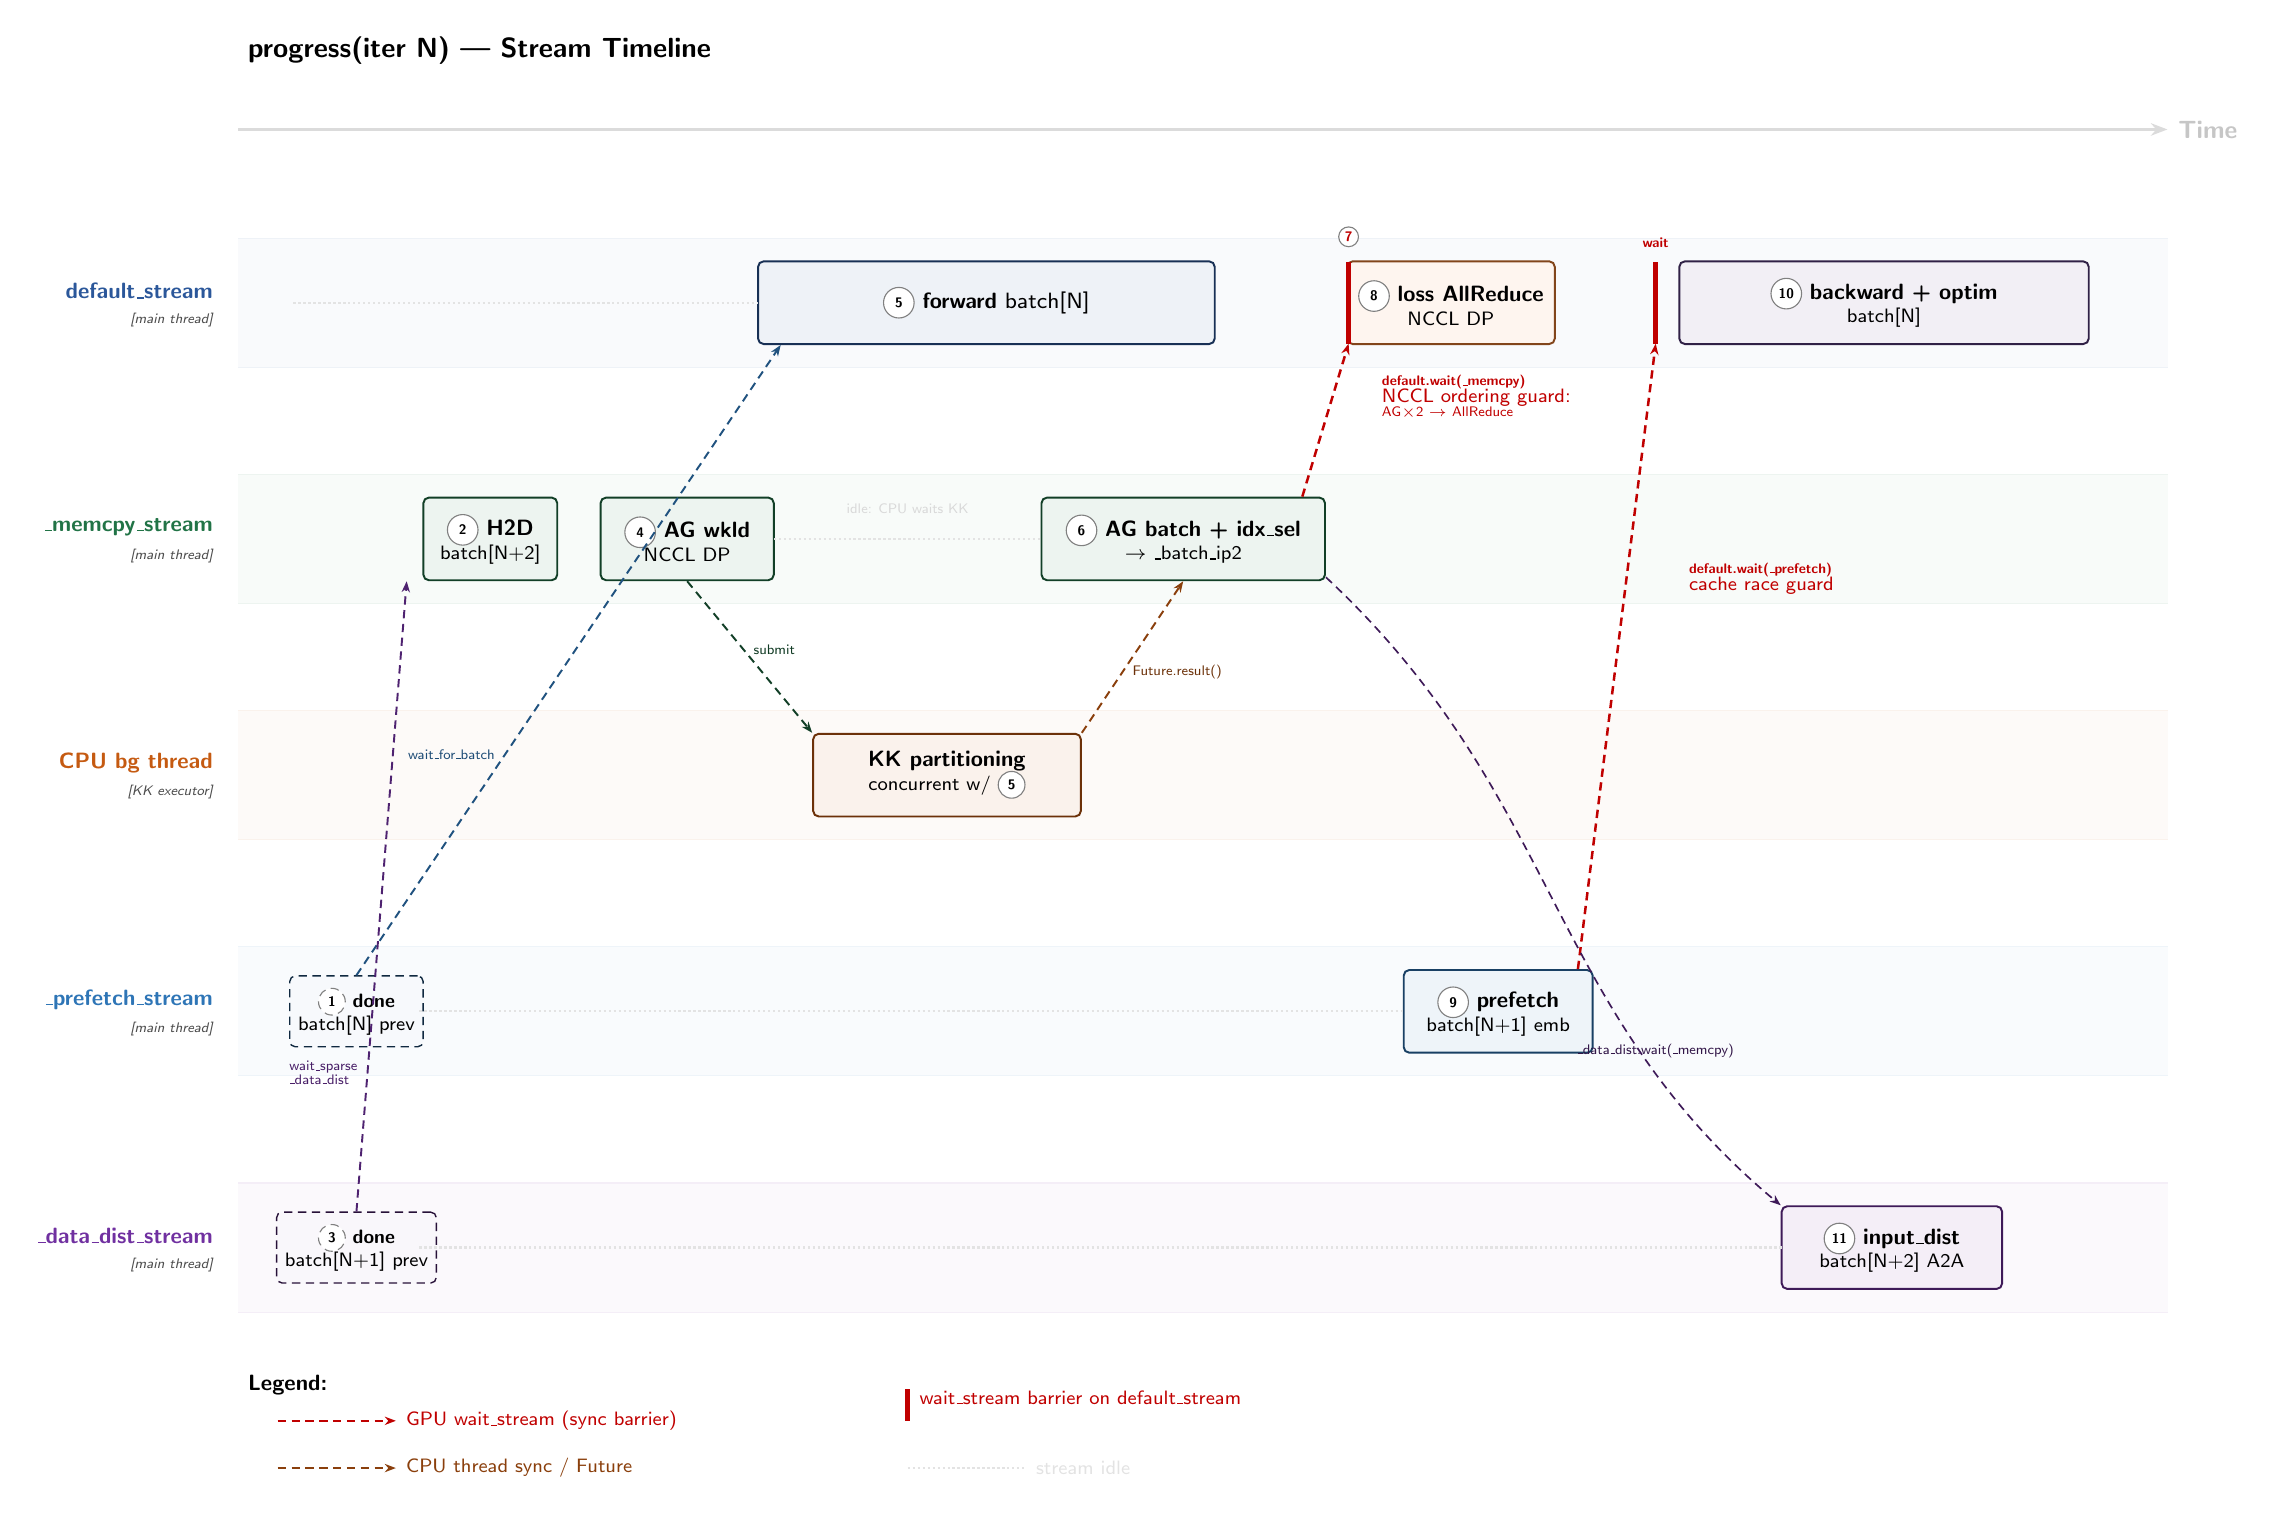
\begin{tikzpicture}[
  op/.style={draw=#1!55!black,fill=#1!8,line width=0.7pt,
    rounded corners=2pt,minimum height=1.05cm,
    inner xsep=4pt,inner ysep=2pt,font=\footnotesize,align=center},
  done/.style={draw=#1!35!black,fill=#1!4,line width=0.5pt,
    rounded corners=2pt,minimum height=0.9cm,
    inner xsep=3pt,inner ysep=2pt,font=\scriptsize,align=center,
    densely dashed},
  sa/.style={-{Stealth[length=4pt,width=3pt]},densely dashed,
    line width=0.7pt,#1},
  sa/.default={cSync},
  lbl/.style={font=\footnotesize\bfseries,text=#1,anchor=east},
  sub/.style={font=\tiny\itshape,text=gray!60!black,anchor=east},
  an/.style={font=\tiny,text=#1,align=left},
]

%% ===== Lane Y positions =====
\def\Yd{12}\def\Ym{9}\def\Yc{6}\def\Yp{3}\def\Yi{0}

%% ===== lane backgrounds =====
\begin{scope}[on background layer]
  \foreach \y/\c in {\Yd/cDef,\Ym/cMem,\Yc/cCpu,\Yp/cPre,\Yi/cDat}{
    \fill[\c!3](-0.5,\y-0.82) rectangle (24,\y+0.82);
    \draw[\c!8,thin](-0.5,\y+0.82)--(24,\y+0.82);
    \draw[\c!8,thin](-0.5,\y-0.82)--(24,\y-0.82);
  }
\end{scope}

%% ===== stream labels =====
\node[lbl=cDef] at (-0.7,\Yd+0.15){default\_stream};
\node[sub]      at (-0.7,\Yd-0.22){[main thread]};
\node[lbl=cMem] at (-0.7,\Ym+0.15){\_memcpy\_stream};
\node[sub]      at (-0.7,\Ym-0.22){[main thread]};
\node[lbl=cCpu] at (-0.7,\Yc+0.15){CPU bg thread};
\node[sub]      at (-0.7,\Yc-0.22){[KK executor]};
\node[lbl=cPre] at (-0.7,\Yp+0.15){\_prefetch\_stream};
\node[sub]      at (-0.7,\Yp-0.22){[main thread]};
\node[lbl=cDat] at (-0.7,\Yi+0.15){\_data\_dist\_stream};
\node[sub]      at (-0.7,\Yi-0.22){[main thread]};

%% ===== time arrow =====
\draw[-{Stealth[length=6pt]},very thick,gray!28]
  (-0.5,14.2)--(24,14.2) node[right,font=\small\bfseries,text=gray!45]{Time};

%% ===== title =====
\node[font=\normalsize\bfseries,anchor=west] at (-0.5,15.2)
  {progress(iter N) --- Stream Timeline};

%% =====================================================
%%  OPERATION BOXES
%% =====================================================

%% -- default_stream --
\node[op=cDef,minimum width=5.8cm](fwd) at(9,\Yd)
  {\cn{5} \textbf{forward} batch[N]};
\node[op=cOra,minimum width=2.2cm](loss) at(14.9,\Yd)
  {\cn{8} \textbf{loss AllReduce}\\[-1pt]\scriptsize NCCL DP};
\node[op=cDef!70!purple,minimum width=5.2cm](bwd) at(20.4,\Yd)
  {\cn{10} \textbf{backward + optim}\\[-1pt]\scriptsize batch[N]};

% idle before forward
\draw[gray!22,densely dotted,line width=0.8pt](0.2,\Yd)--(6.1,\Yd);

%% -- barriers on default_stream --
% barrier 7: default.wait_stream(_memcpy)
\draw[cSync,line width=2pt](13.6,\Yd-0.52)--(13.6,\Yd+0.52);
\node[above,font=\tiny\bfseries,text=cSync] at(13.6,\Yd+0.58){\cn{7}};

% barrier: default.wait_stream(_prefetch), before backward
\draw[cSync,line width=2pt](17.5,\Yd-0.52)--(17.5,\Yd+0.52);
\node[above,font=\tiny\bfseries,text=cSync] at(17.5,\Yd+0.58){wait};

%% -- _memcpy_stream --
\node[op=cMem,minimum width=1.7cm](h2d) at(2.7,\Ym)
  {\cn{2} \textbf{H2D}\\[-1pt]\scriptsize batch[N+2]};
\node[op=cMem,minimum width=2.2cm](agw) at(5.2,\Ym)
  {\cn{4} \textbf{AG wkld}\\[-1pt]\scriptsize NCCL DP};
\node[op=cMem,minimum width=3.6cm](fin) at(11.5,\Ym)
  {\cn{6} \textbf{AG batch + idx\_sel}\\[-1pt]\scriptsize $\to$ \_batch\_ip2};

% idle gap (CPU blocks on KK Future)
\draw[gray!22,densely dotted,line width=0.8pt](6.3,\Ym)--(9.7,\Ym);
\node[font=\tiny,text=gray!30] at(8,\Ym+0.38){idle: CPU waits KK};

%% -- CPU bg thread --
\node[op=cCpu,minimum width=3.4cm](kk) at(8.5,\Yc)
  {\textbf{KK partitioning}\\[-1pt]\scriptsize concurrent w/ \cn{5}};

%% -- _prefetch_stream --
\node[done=cPre,minimum width=1.6cm](ppf) at(1.0,\Yp)
  {\cn{1} \textbf{done}\\[-1pt]\scriptsize batch[N] prev};
\node[op=cPre,minimum width=2.4cm](pf) at(15.5,\Yp)
  {\cn{9} \textbf{prefetch}\\[-1pt]\scriptsize batch[N+1] emb};
\draw[gray!22,densely dotted,line width=0.8pt](1.8,\Yp)--(14.3,\Yp);

%% -- _data_dist_stream --
\node[done=cDat,minimum width=1.6cm](pdd) at(1.0,\Yi)
  {\cn{3} \textbf{done}\\[-1pt]\scriptsize batch[N+1] prev};
\node[op=cDat,minimum width=2.8cm](inp) at(20.5,\Yi)
  {\cn{11} \textbf{input\_dist}\\[-1pt]\scriptsize batch[N+2] A2A};
\draw[gray!22,densely dotted,line width=0.8pt](1.8,\Yi)--(19.1,\Yi);

%% =====================================================
%%  SYNC ARROWS
%% =====================================================

%% --- 1  _prefetch -> default  (wait_for_batch) ---
\draw[sa=cPre!70!black]
  (ppf.north) --
  node[left,an=cPre!65!black,pos=0.35]{wait\_for\_batch}
  ($(fwd.south west)+(0.3,0)$);

%% --- 3  _data_dist -> memcpy area  (wait_sparse_data_dist) ---
\draw[sa=cDat!70!black]
  (pdd.north) --
  node[left,an=cDat!65!black,pos=0.22]{wait\_sparse\\[-1pt]\_data\_dist}
  ($(h2d.south west)+(-0.2,0)$);

%% --- 4 -> KK  (submit to executor) ---
\draw[sa=cMem!55!black]
  (agw.south) --
  node[right,an=cMem!50!black,pos=0.45]{submit}
  (kk.north west);

%% --- KK -> 6  (Future.result) ---
\draw[sa=cCpu!70!black]
  (kk.north east) --
  node[right,an=cCpu!55!black,pos=0.4]{Future.result()}
  ($(fin.south)+(0,0)$);

%% --- 7  _memcpy -> default  (wait_stream, NCCL ordering guard) ---
\draw[sa,line width=0.9pt]
  ($(fin.north east)+(-0.3,0)$) -- (13.6,\Yd-0.52);
\node[an=cSync,right] at(13.9,10.8)
  {\textbf{default.wait(\_memcpy)}\\[-1pt]
   \mdseries\scriptsize NCCL ordering guard:\\[-1pt]
   AG$\times$2 $\to$ AllReduce};

%% --- _prefetch -> default  (wait_stream, cache race guard) ---
\draw[sa,line width=0.9pt]
  ($(pf.north east)+(-0.2,0)$) -- (17.5,\Yd-0.52);
\node[an=cSync,right] at(17.8,8.5)
  {\textbf{default.wait(\_prefetch)}\\[-1pt]
   \mdseries\scriptsize cache race guard};

%% --- 11  _memcpy -> _data_dist  (internal wait_stream) ---
\draw[sa=cDat!55!black,line width=0.6pt]
  ($(fin.south east)+(0,0.05)$)
  .. controls +(3,-2.8) and +(-3,2.5) ..
  (inp.north west);
\node[an=cDat!45!black] at(17.5,2.5)
  {\_data\_dist.wait(\_memcpy)};

%% =====================================================
%%  LEGEND
%% =====================================================
\node[anchor=north west,font=\footnotesize\bfseries] at(-0.5,-1.5){Legend:};

\draw[sa=cSync,line width=0.8pt](0,-2.2)--(1.5,-2.2)
  node[right,font=\scriptsize]{GPU wait\_stream (sync barrier)};
\draw[sa=cCpu!70!black,line width=0.8pt](0,-2.8)--(1.5,-2.8)
  node[right,font=\scriptsize]{CPU thread sync / Future};

\draw[cSync,line width=2pt](8,-2.2)--(8,-1.8)
  node[right,font=\scriptsize,yshift=-3pt]{wait\_stream barrier on default\_stream};
\draw[gray!22,densely dotted,line width=0.8pt](8,-2.8)--(9.5,-2.8)
  node[right,font=\scriptsize]{stream idle};

\end{tikzpicture}
\end{document}
